\begin{exercise}
Draw pictures of \(\Spec(\mathbf Z)\), \(\Spec(\mathbf R)\), \(\Spec(\mathbf C[x])\), \(\Spec(\mathbf R[x])\), and \(\Spec(\mathbf Z[x])\).
\end{exercise}

\begin{solution}
We draw inspiration from \cite[Chapter~II]{EisenbudHarrisGeometryOfSchemes},  \cite[Chapter~II,~\S1]{MumfordRedBook}, and \cite[Chapter~3]{VakilNotes}.

\begin{enumerate}
\item
The ring \(\mathbf{Z}\) is a principal ideal domain whose prime/irreducible elements are, up to a multiple of \(-1\), exactly the positive prime integers.
Consequently, the prime ideals of \(\mathbf{Z}\) are the maximal ideals \((p)\) for positive prime numbers \(p\), and the zero ideal \((0)\).

\autoref{fig:Spec(Z)} is a picture of \(\Spec(\mathbf{Z})\).

\begin{figure}
\centering
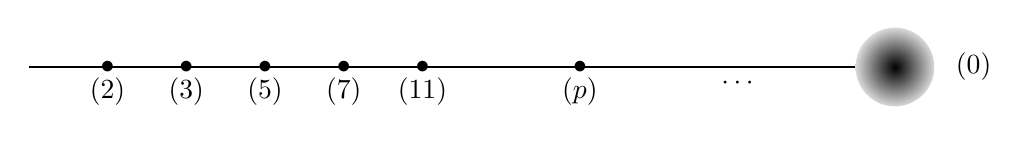
\begin{tikzpicture}
% Non-zero primes (closed points)
\draw[thick] (0,0)
    -- (1,0) node {\(\bullet\)} node[below] {\((2)\)}
    -- (2,0) node {\(\bullet\)} node[below] {\((3)\)}
    -- (3,0) node {\(\bullet\)} node[below] {\((5)\)}
    -- (4,0) node {\(\bullet\)} node[below] {\((7)\)}
    -- (5,0) node {\(\bullet\)} node[below] {\((11)\)}
    -- (7,0) node {\(\bullet\)} node[below] {\((p)\)}
    -- (9,0) node[below] {\(\cdots\)}
    -- (11,0);
% Generic point
\shade[inner color=black, outer color=gray!30]
    (11,0) circle (0.5);
\draw (12,0) node {\((0)\)};
\end{tikzpicture}
\caption{%
\(\Spec(\mathbf{Z})\) consists of a closed point \((p)\) for each positive prime number \(p\), as well as a generic point corresponding to the minimal prime ideal \((0)\).%
}
\label{fig:Spec(Z)}
\end{figure}

\item
The only prime ideal of the field \(\mathbf{R}\) is the zero ideal.
Thus, \(\Spec(\mathbf{R})\) consists of a single point: \(\bullet\).
In fact, for any ring \(A\), the space \(\Spec(A)\) consists of a single point if and only if \(A\) is a field.
\item
The polynomial ring \(\mathbf{C}[x]\) is a principal ideal domain, so its non-zero prime ideals are maximal and generated by monic, irreducible polynomials.
Since \(\mathbf{C}\) is algebraically closed, these polynomials are of the form \(x - a\) for \(a \in \mathbf{C}\).
Also, the zero ideal \((0)\) is prime and is a generic point of \(\Spec(\mathbf{C}[x])\).

If we identify the closed points of \(\Spec(\mathbf{C}[x])\) (i.e., maximal ideals of \(\mathbf{C}[x]\)) with complex numbers via the correspondence \((x - a) \leftrightarrow a\), then the subspace topology on the set of closed points of \(\Spec(\mathbf{C}[x])\) coincides with the classical Zariski topology on the affine line \(\mathbf{A}_{\mathbf{C}}^1 = \mathbf{C}\), in which the closed sets are sets on which a polynomial in one variable with complex coefficients vanishes (which, in the one-dimensional case, happens to be the cofinite topology).

\autoref{fig:Spec(C[x])} is a picture of \(\Spec(\mathbf{C}[x])\).

\begin{figure}
\centering
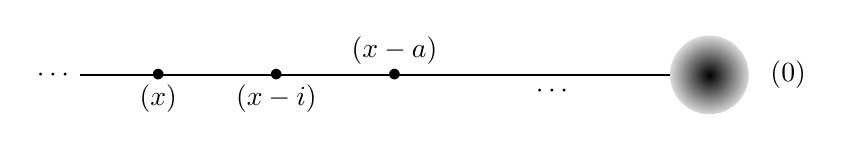
\begin{tikzpicture}
% Non-zero primes (closed points)
\draw[thick] (0,0) node[left] {\(\cdots\)}
    -- (1,0) node {\(\bullet\)} node[below] {\((x)\)}
    -- (2.5,0) node {\(\bullet\)} node[below] {\((x - i)\)}
    -- (4,0) node {\(\bullet\)} node[above] {\((x - a)\)}
    -- (6,0) node[below] {\(\cdots\)}
    -- (8,0);
% Generic point
\shade[inner color=black, outer color=gray!30]
    (8,0) circle (0.5);
\draw (9,0) node {\((0)\)};
\end{tikzpicture}
\caption{%
\(\Spec(\mathbf{C[x]})\) is the one-dimensional complex affine line consisting of a closed point \((x - a)\) for each \(a \in \mathbf{C}\), as well as a generic point corresponding to the minimal prime ideal \((0)\).%
}
\label{fig:Spec(C[x])}
\end{figure}

\item
The non-zero prime ideals of \(\mathbf R[x]\) correspond to monic irreducible polynomials over \(\mathbf R\).
These are either of the form \(x - a\) with \(a \in \mathbf R\), or of the form \(x^2 + bx + c\), with \(b^2 - 4c < 0\).
Each polynomial of the latter type corresponds to two conjugate complex numbers with non-zero imaginary part, the roots of the polynomial.
Thus \(\Spec(\mathbf R[x])\) can be seen as the complex plane folded along the real axis (or with conjugate points identified), together with an extra generic point, the zero ideal.

\autoref{fig:Spec(R[x])} is a picture of \(\Spec(\mathbf{R}[x])\).

\begin{figure}
\centering
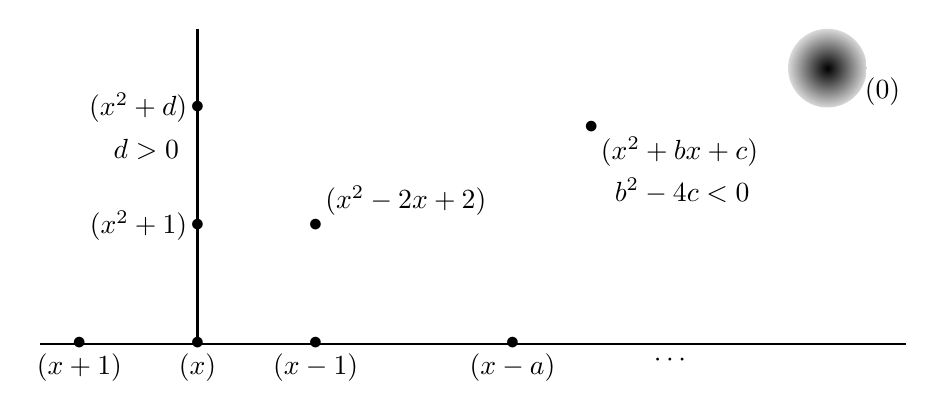
\begin{tikzpicture}
\draw[thick] (-1,0)
    -- (-0.5,0) node {$\bullet$} node[below] {$(x+1)$}
    -- (1,0) node {$\bullet$} node[below] {$(x)$}
    -- (2.5,0) node {$\bullet$} node[below] {$(x-1)$}
    -- (5,0) node {$\bullet$} node[below] {$(x-a)$}
    -- (7,0) node[below] {$\cdots$}
    -- (10,0);
\draw[thick] (1,0)
    -- (1,1.5) node {$\bullet$} node[left] {$(x^2 + 1)$}
    -- (1,3) node {$\bullet$} node[left] {$(x^2 + d)$} node[left, yshift=-15, xshift=-3] {$d > 0$}
    -- (1,4);
\draw (2.5,1.5) node {$\bullet$} node[above right] {$(x^2 - 2x + 2)$};
\draw (6,2.75) node {$\bullet$} node[below right] {$(x^2 + bx + c)$} node[below right, yshift=-15, xshift=5] {$b^2 - 4c < 0$};
\shade[inner color=black, outer color=gray!30] (9,3.5) circle (0.5);
\draw (9.7,3.2) node {$(0)$};
\end{tikzpicture}
\caption{%
\(\Spec(\mathbf{R}[x])\) can be visualized as the complex plane folded along the real axis, together with an extra generic point.%
}
\label{fig:Spec(R[x])}
\end{figure}

\item
The non-zero prime ideals of \(\mathbf{Z}[x]\) are of two forms.
First, there are the principle prime ideals \((f)\), where either \(f \in \mathbf{Z}\) is a positive prime number or \(f \in \mathbf{Z}[x]\) is a \(\mathbf{Q}\)-irreducible polynomial written with coefficients reduced to have g.c.d. \(= 1\).
Second, there are the maximal ideals, which are of the form \((p, f)\), where \(p\) is a positive prime integer and \(f \in \mathbf{Z}[x]\) is a monic polynomial which is irreducible modulo \(p\).

\autoref{fig:Spec(Z[x])} is a picture of \(\Spec(\mathbf{Z}[x])\) taken from \cite[Chapter~2, \S1, Example~H]{MumfordRedBook}.

\begin{figure}
\centering
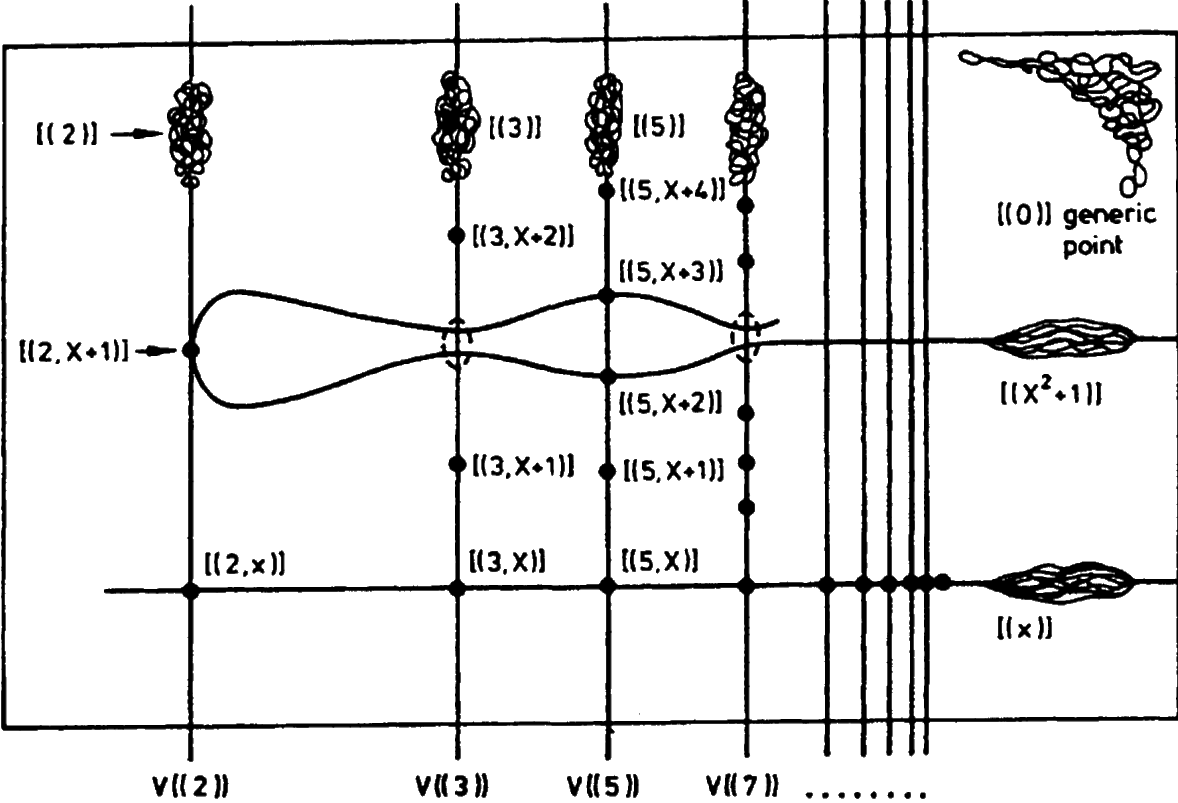
\includegraphics[width=0.9\textwidth]{images/Spec(Z[x]).png}
\caption{%
Picture of \(\Spec(\mathbf{Z}[x])\) taken from \cite[Chapter~2, \S1, Example~H]{MumfordRedBook}%
}
\label{fig:Spec(Z[x])}
\end{figure}
\end{enumerate}
\let\qed\relax
\end{solution}